\subsection{Aufbau}
Der hier verwendete Aufbau ist in Abb. \ref{fig:aufbau} zu sehen.
\begin{figure}
  \centering
  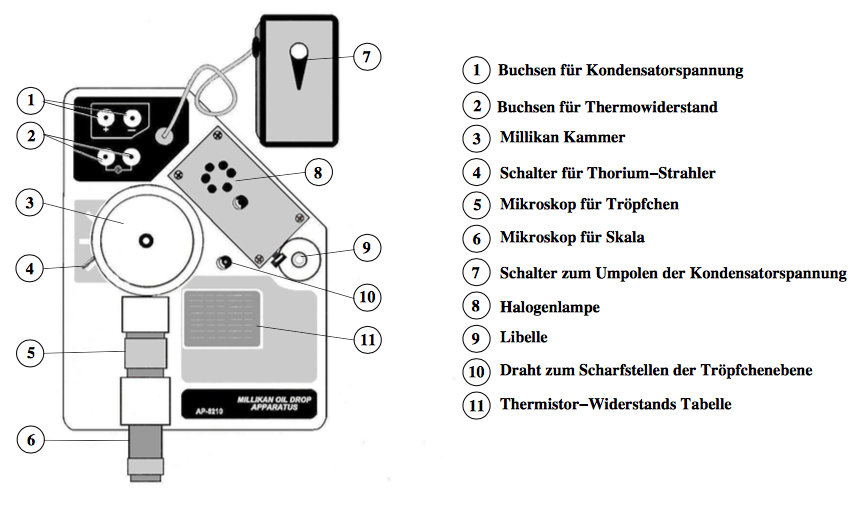
\includegraphics[width=0.8\textwidth]{bilder/aufbau.png}
  \caption{Aufbau für den Millikan-Versuch \cite{503}}
  \label{fig:aufbau}
\end{figure}
In einer Kammer befindet sich ein Plattenkondensator mit einem Plattenabstand
$d=(7.659\pm0.0051)\mm$. Die obere Platte besitzt ein Loch in der Mitte, durch
das die Öltröpfchen mit $\rho_\su{Öl}=886 \,\si{\kilo\gram\per\cubic\meter}$
durch die Zerstäubung in den Kondensator gelangen. Eine Halogenlampe macht die
Tröpfchen unter einem Mikroskop sichtbar. Um das Mikroskop scharf zu stellen wird
die Justiernadel $10$ aus der Halterung geschraubt und auf den Deckel der Millikankammer $3$
gesteckt. Anschließend wird das Mikroskop $5$ auf die Nadel fokussiert und mit $6$
kann das Raster ($1$ Einheit = $0.5\mm$) zum scharf stellen benutzt werden. Danach wird
die Nadel in ihre Halterung zurückgeschraubt. Mit einem Thermowiderstand wird ständig
die Temperatur der Luft in der Kammer kontrolliert, da sie sich aufgrund der Halogenlampe
erwärmt. Der Widerstand des Thermistors wird an den Buchsen $2$ gemessen. Die Umrechnung
von Widerstand in Temperatur ist in Tabelle \ref{tab:tabelle} zu finden.
\begin{figure}
  \centering
  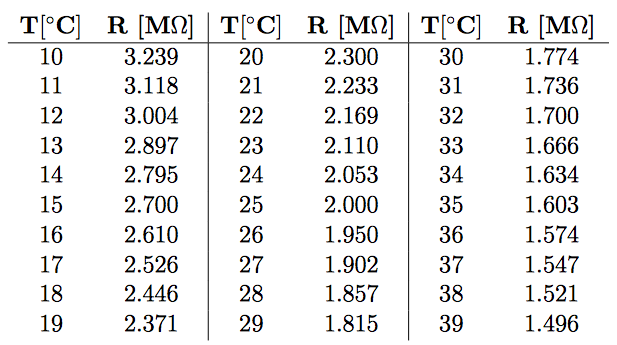
\includegraphics[width=0.6\textwidth]{bilder/tabelle.png}
  \caption{Umrechnung Thermowiderstand in Temperatur \cite{503}}
  \label{tab:tabelle}
\end{figure}
Um die elektrische Ladung
der Tröpfchen zu verändern wird ein schwach radioaktives $\alpha$ - Präparat
($\ce{^{232}Th}, 8 \mu Ci$) verwendet, welches sich in der unteren Kondensatorplatte
befindet. Mit Hebel $4$ kann dies durchgeführt werden.
Vor der Durchführung wird mit einer Libelle $9$ überprüft, ob die Apparatur
waagerecht ist. Mit Hebel $7$ wird das elektrische Feld angelegt.

\subsection{Bestimmung der Elementarladung}
Zuerst wird ein wenig Öl in die Kammer gesprüht. Das $\vec{E}$ - Feld ist dabei
ausgeschaltet. Dann wird ein Tröpfchen ausgewählt, dass eine Geschwindigkeit von
$v = 0.001\,\si{\centi\meter\per\second}$ bis $v = 0.01\,\si{\centi\meter\per\second}$
besitzt. Mit Hebel $7$ wird dann kurz das elektrische Feld angelegt, um zu überprüfen,
ob das Tröpfchen auch geladen ist. Ist dies nicht der Fall, so wird das Feld wieder
ausgeschaltet und mit Hebel $4$ wird die radioaktive Quelle eingeschaltet, um die
Umgebungsluft zu ionisieren, wodurch sich mehr Elementarladungen auf dem Tröpfchen
anlagern. Wenn das Teilchen nun geladen ist, so wird das elektrische Feld wieder
eingeschaltet und es wird die Zeit $t_\su{auf}$ gemessen, die das Teilchen zum zurücklegen einer
bestimmten Strecke benötigt. Anschließend wird das Feld umgepolt und es wird erneut
die Zeit $t_\su{ab}$ gemessen, die das Teilchen benötigt, um die gleiche Strecke wieder
zurückzufliegen. Um die Messungenauigkeiten so gering wie möglich zu halten, sollten die
Steiggeschwindigkeit $v_\su{auf}$ und die Sinkgeschwindigkeit $v_\su{ab}$ ständig
bestimmt werden. Abschließend wird die Gleichgewichtsgeschwindigkeit $v_0$ bei
ausgeschaltetem elektrischen Feld gemessen. Die Messung wird dann für mehrere
Tröpfchen immer wieder durchgeführt.

Ist dieser Vorgang beendet, so wird er für 4 weitere Kondensatorspannungen
wiederholt. Dabei darf die Spannung $U=500\Volt$ nicht überschritten werden.
